\documentclass[12pt,a4paper]{article}
\usepackage[utf8]{inputenc}
\usepackage{amsmath}
\usepackage{textcomp}

\usepackage{geometry}
\geometry{a4paper,left=25mm,right=25mm, top=2cm, bottom=2cm} 

\usepackage{verbatim}

 \usepackage{mathptmx}
 \usepackage[scaled=.90]{helvet}
 \usepackage{courier}

\usepackage[utf8]{inputenc}

\usepackage{listings}
\usepackage{color}

\usepackage{graphicx}
 
\definecolor{dkgreen}{rgb}{0,0.6,0}
\definecolor{gray}{rgb}{0.5,0.5,0.5}
\definecolor{mauve}{rgb}{0.58,0,0.82}

\pagestyle{empty}
\lstset{numbers=left,language=C++}
\lstset{showstringspaces=false,
basicstyle=\ttfamily\footnotesize,
breaklines=true,
tabsize=3,
commentstyle=\color{dkgreen},       % comment style
}

%keine einrückungen bei absatz
\parindent 0pt

\begin{document}
\title{Übung 2}
\author{Bernhard Selymes, Reinhard Penn}
\date{November 2012}

\normalsize

%Pfad zu c++ Dateien
\newcommand{\CodePath}{../AdressManagment/AdressManagement/}

%Beginn des Dokuments
\section{Organisatorisches}

\subsection{Team}
	\begin {itemize} 
		\item Reinhard Penn, s1110306019 
		\item Bernhard Selymes, s1110306024
	\end {itemize}

\subsection{Aufteilung}
	\begin {itemize} 
		\item Reinhard Penn
			\begin {itemize}
				\item Planung
				\item Klassendiagramm
				\item Implementierung der Klassen AdressManager, Writer, AsciiWriter, HtmlWriter, Person, Adress
				\item Testen alle Klassen
			\end {itemize}
		\item Bernhard Selymes
			\begin {itemize}
				\item Planung
				\item Klassendiagramm
				\item Implementierung der Klassen Reader, PersonReader, AdressReader, Person, Adress
				\item Dokumentation				
			\end {itemize}
	\end {itemize}


\subsection{Zeitaufwand}
	\begin {itemize}
		\item geschätzte Mh: 7h
		\item tatsächlich: Reinhard (10h), Bernhard  (10h)
	\end {itemize}


\section{Systemspezifikation}
Es soll eine Software für die Verwaltung von Adressen und Personen erstellt werden. Die Daten werden aus verschiedenen Dateien eingelesen, danach werden sie verlinkt und können dann als Html- oder Acsii-Datei ausgegeben werden.
\newline
In beiden Dateien gibt es einen Header der überlesen werden kann. Die Einlesenreihenefolge der Dateien ist beliebig. Eine Personendatei enthält den Namen und Index von den Personen, eine Adressdatei Straße, Hausnummer, PLZ und Ort. Die Reihenfolge der Adressen gibt deren Index an.
 \\


\newpage
\section {Systementwurf}

\subsection {Klassendiagramm}

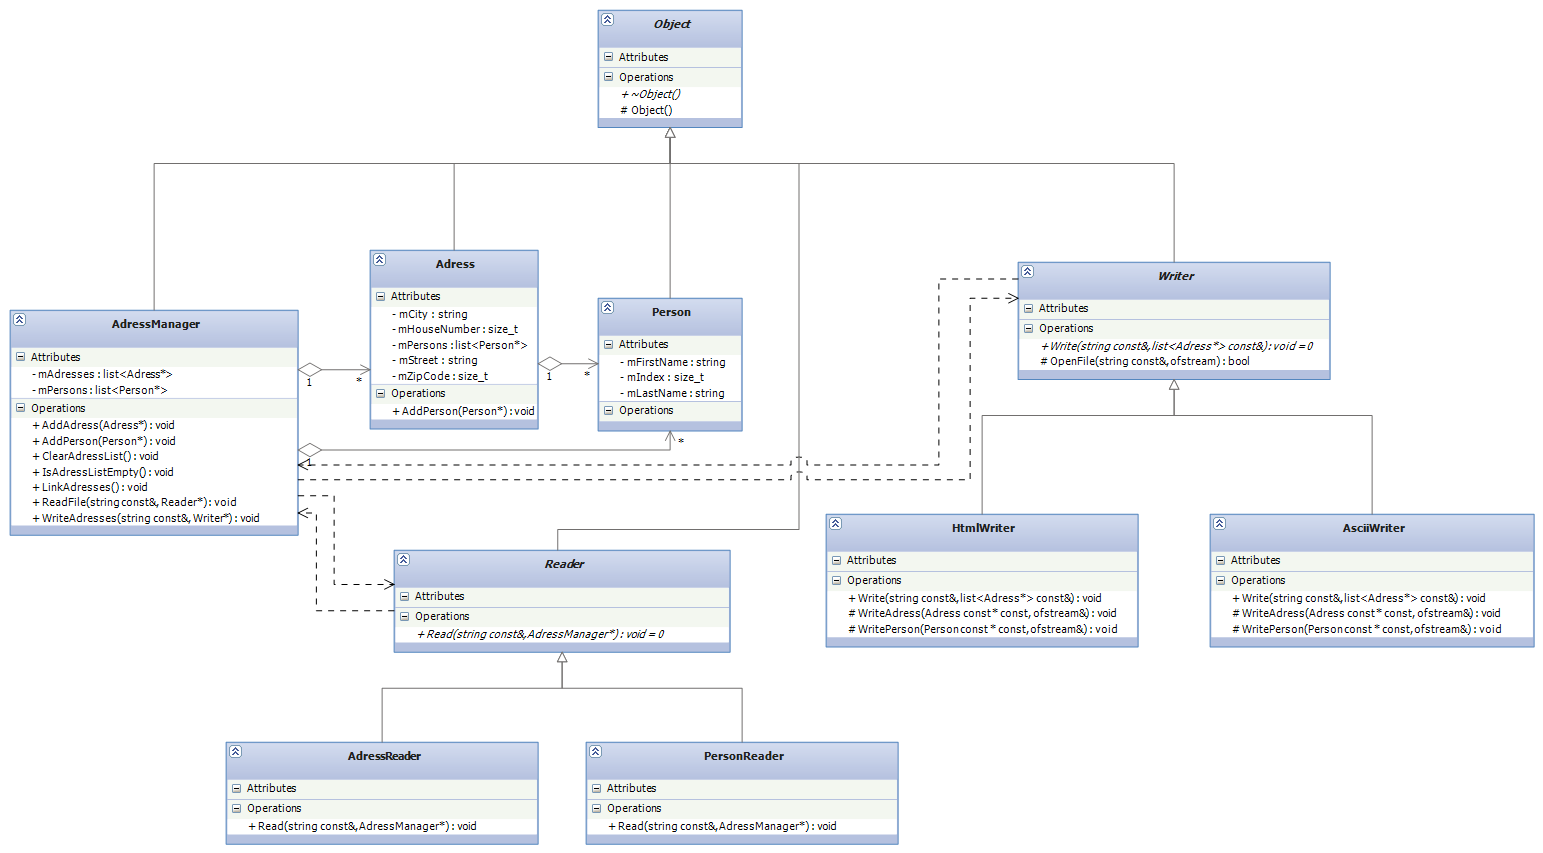
\includegraphics[angle=90,scale=0.6] {../Klassendiagramm.png}

\newpage
\subsection {Komponentenübersicht}
\begin {itemize} 
	\item Klasse "Object":
	\newline
	Basis aller Basisklassen.
	\item Klasse "AdressManager":
	\newline
	Beinhaltet die eingelesene Adressen und Personen und kann diese verlinken.
	\item Klasse "Adress":
	\newline	
	Beinhalten die Daten einer Adresse und zusätzlich die Personen die in dieser Adresse wohnen.
	\item Klasse "Person":
	\newline
	Beinhaltet die Daten einer Person.
	\item Klasse "Writer":
	\newline
	Abstrakte Basisklasse.
	\item Klasse "HtmlWriter": 
	\newline
	Wird von "Writer" abgeleitet, gibt die Daten in einer Html-Datei aus.
	\item Klasse "AsciiWriter":
	\newline
	Wird von "Writer" abgeleitet, gibt die Daten in einer Ascii-Datei aus.
	\item Klasse "Reader"
	\newline
	Abstrakte Basisklasse.
	\item Klasse "AdressReader"
	\newline
	Wird von "Reader" abgeleitet, liest die Adressen ein.
	\item Klasse "PersonReader"
	\newline
	Wird von "Reader" abgeleitet, liest die Personen ein.
	
\end {itemize}

\newpage
\section {Komponentenentwurf}
\subsection {Klasse "Object"}
Abstrakte Basisklasse aller Klassen. Von ihr werden alle anderen Klassen abgeleitet. Beinhaltet einen virtuellen Destruktor.

\subsection {Klasse "AdressManager"}
Hat zwei Listen in denen Zeiger von Adressen und Personen gespeichert werden.
 \\

\textbf {Methode "AddAdress": } 
\newline
Schnittstelle: Parameter: Adress*. Rückgabetyp: void.
\newline 
Fügt der Liste via pushback neue Adressen hinzu.\\

\textbf {Methode "AddPerson": } 
\newline
Schnittstelle: Parameter: Person*. Rückgabetyp: void.
\newline
Fügt der Liste via pushback neue Personen hinzu. \\

\textbf {Methode "LinkAdresses": } 
\newline
Schnittstelle: Rückgabetyp: void.
\newline
 Geht die Liste mit den Personen durch und fügt sie bei der entsprechenden Adresse ein. Löscht alle Personen die keiner Adresse hinzugefügt werden können. \\

\textbf {Methode "ReadFile": } 
\newline
Schnittstelle: Parameter: string const\& , Reader*. Rückgabetyp: void.
\newline
Liest Daten mithilfe eines Readers ein.
\\

\textbf {Methode "WriteFile": } 
\newline
Schnittstelle: Parameter: string const\& , Writer*. Rückgabetyp: void.
\newline
Gibt Daten mithilfe eines Writers aus.
\\

\textbf {Methode "ClearAdressList": } 
\newline
Schnittstelle: Rückgabetyp: void.
\newline 
Löscht die Objekte aus der Liste mit den Adressen.\\


\subsection {Klasse "Adress"}
Hat folgende Member: ZipCode, City, Street, HouseNumber, Liste mit Personen. Hat für alle eine set- und eine get-Funktion.\\

\textbf {Methode "AddPerson": } 
\newline
Schnittstelle: Parameter: Person*. Rückgabetyp: void.
\newline
Fügt der Liste mit den Personen eine Person hinzu.
\\

\subsection {Klasse "Person"}
Hat folgender Member: FirstName, LastName, Index. Getter und Setter für alle Member. \\

\subsection {Klasse "Reader"}
\textbf {Methode "Read":}
\newline
Schnittstelle: Parameter: string const \&, AdressManager*. Rückgabetyp: void.
\newline
Pure virtual function, die nur die Schnittstelle definiert und nicht implementiert ist. \\

\subsection {Klasse "AdressReader" und Klasse "PersonReader"}
Der Unterschied der beiden Klassen liegt nur darin, dass sich die Daten die eingelesen werden unterscheiden. \\
\newline
\textbf {Methode "Read":}
\newline
Schnittstelle: Parameter: string const \&, AdressManager*. Rückgabetyp: void.
\newline
Liest mithilfe der getline Funktion Zeile für Zeile Daten aus einer Textdatei. Der Header der Datei wird überlesen. Aus dem String den die getline Funktion liefert, werden die Daten mithilfe verschiedenster string-Funktionen (find\_first\_of, substr, erase) extrahiert. Zahlen werden mithilfe eines stringstreams in ein size\_t umgewandelt.  Die Objekte werden in dieser Funktion erzeugt und befüllt und auch gleich zum AdressManager hinzugefügt. Wir haben definiert, dass die Struktur der Daten eingehalten werden muss, wenn falsche Daten in falscher Reihenfolge in der Datei sind, dann werden irgendwelche undefinierte oder zufällige Werte gespeichert. \\

\subsection {Klasse "Writer"}
\textbf {Methode "Write":}
\newline
Schnittstelle: Parameter: string const \&, TAdresses const\&. Rückgabetyp: void.
\newline
Pure virtual function, die nur die Schnittstelle definiert und nicht implementiert ist. \\
\newline
\textbf {Methode "OpenFile":}
\newline
Schnittstelle: Parameter: string const \&, ofstream\&. Rückgabetyp: bool.
\newline
Gibt zurück ob die Datei geöffnet werden konnte oder nicht. \\

\subsection {Klasse "HtmlWriter" und "AsciiWriter"}
Die beiden Klassen unterscheiden sich nur in der Formatierung der Ausgabedateien. \\
\newline
\textbf {Methode "Write":}
\newline
Schnittstelle: Parameter: string const \&, TAdresses const\&. Rückgabetyp: void.
\newline
Schreibt Daten in eine Ascii/Html-Datei. Dabei wird die Hilfsfunktion "WriteAdresses" verwendet. Beim HtmlWriter wird die Formatierung dadurch erreicht, dass Html-Befehle in den filestream geschrieben werden.\\
\textbf {Methode "WriteAdresses":}
\newline
Schreibt die Adressdaten mit der entsprechenden Formatierung in die Datei. Ruft für alle Personen die in dieser Adresse wohnen "WritePerson" auf. \\
\textbf {Methode "WritePersons":}
\newline
Schreibt die Personendaten mit der entsprechenden Formatierung in die Datei. \\

\newpage
\section {Source Code}

\lstinputlisting[language=C++]{\CodePath Object.h}
\lstinputlisting[language=C++]{\CodePath Object.cpp}

\newpage
\lstinputlisting[language=C++]{\CodePath AdressManager.h}
\newpage
\lstinputlisting[language=C++]{\CodePath AdressManager.cpp}

\newpage
\lstinputlisting[language=C++]{\CodePath Adress.h}

\newpage
\lstinputlisting[language=C++]{\CodePath Person.h}

\newpage
\lstinputlisting[language=C++]{\CodePath Writer.h}
\newpage
\lstinputlisting[language=C++]{\CodePath Writer.cpp}

\newpage
\lstinputlisting[language=C++]{\CodePath HtmlWriter.h}
\newpage
\lstinputlisting[language=C++]{\CodePath HtmlWriter.cpp}

\newpage
\lstinputlisting[language=C++]{\CodePath AsciiWriter.h}
\newpage
\lstinputlisting[language=C++]{\CodePath AsciiWriter.cpp}

\newpage
\lstinputlisting[language=C++]{\CodePath Reader.h}

\newpage
\lstinputlisting[language=C++]{\CodePath PersonReader.h}
\newpage
\lstinputlisting[language=C++]{\CodePath PersonReader.cpp}

\newpage
\lstinputlisting[language=C++]{\CodePath AdressReader.h}
\newpage
\lstinputlisting[language=C++]{\CodePath AdressReader.cpp}

\newpage
\lstinputlisting[language=C++]{\CodePath main.cpp}


\newpage
\section {Testausgaben} 

\begin {verbatim}
Visual Leak Detector Version 2.2.3 installed.
Testcase0: Empty adress file and person files
Read: testcase0_person.txt ... Finished
Read: testcase0_adress.txt ... Finished
LinkAdresses: ... Finished
Write: testcase0_ascii.txt ... Finished
Write: testcase0_html.html ... Finished


Testcase1: Valid adress file(single adress) and empty person files
Read: testcase0_person.txt ... Finished
Read: testcase1_adress.txt ... Finished
LinkAdresses: ... Finished
Write: testcase1_ascii.txt ... Finished
Write: testcase1_html.html ... Finished


Testcase2: 
Valid adress file(single adress) and valid person file(single person)

Read: testcase2_person.txt ... Finished
Read: testcase1_adress.txt ... Finished
LinkAdresses: ... Finished
Write: testcase2_ascii.txt ... Finished
Write: testcase2_html.html ... Finished


Testcase3: 
Valid adress file and valid person file, multiple adresses, persons
Read: testcase3_person.txt ... Finished
Read: testcase3_adress.txt ... Finished
LinkAdresses: ... Finished
Write: testcase3_ascii.txt ... Finished
Write: testcase3_html.html ... Finished


Testcase4: 
Valid adress file and valid person files, multiple adresses, persons
Read: testcase3_person.txt ... Finished
Read: testcase4_person.txt ... Finished
Read: testcase3_adress.txt ... Finished
LinkAdresses: ... Finished
Write: testcase4_ascii.txt ... Finished
Write: testcase4_html.html ... Finished


Testcase5: Corrupted adress file and valid person file
Read: testcase4_person.txt ... Finished
Read: testcase5_adress.txt ... Finished
LinkAdresses: ... Finished
Write: testcase5_ascii.txt ... Finished
Write: testcase5_html.html ... Finished


No memory leaks detected.
Visual Leak Detector is now exiting.
\end {verbatim}


\end{document}